\newpage
\section{Результаты}
\vspace{0.5\baselineskip}

В ходе работы были проведены симуляции динамики кавитационного пузыря в различных условиях, включая воздействие как одиночными, так и тройными лазерными импульсами. При применении одиночного импульса наблюдались начальное формирование, рост кавитационного пузыря и его последующий коллапс. Моделирование позволило зафиксировать ударную волну, возникающую при коллапсе, а также сравнить динамику кавитационного пузыря с экспериментальными данными.

\begin{figure}[h!]
    \centering
    % First row
    \begin{subfigure}{.45\textwidth}
        
\includegraphics[width=\textwidth]{1_1.png}
    \end{subfigure}
    \hspace{1cm}
    \begin{subfigure}{.45\textwidth}
        
\includegraphics[width=\textwidth]{1_2.png}
    \end{subfigure}
    
    % Second row
    \vspace{1em} % Space between rows
    \begin{subfigure}{.45\textwidth}
        
\includegraphics[width=\textwidth]{1_3.png}
    \end{subfigure}
    \hspace{1cm}
    \begin{subfigure}{.45\textwidth}
        
\includegraphics[width=\textwidth]{1_4.png}
    \end{subfigure}

    \hspace{5pt}
    \caption{\centering Динамика кавитационного пузыря, вызванного одиночным лазерным импульсом}
    \label{fig:single_impulse}
\end{figure}

При моделировании кавитационного, индуцированного одиночным лазерным импульсом, явно наблюдается рост и коллапс с дальнейшим его сокращением.

\begin{comment}
\begin{figure}[h!]
    \centering
    % First row
    \begin{subfigure}{.45\textwidth}
        
\includegraphics[width=\textwidth]{3_1.png}
    \end{subfigure}
    \hspace{1cm}
    \begin{subfigure}{.45\textwidth}
        
\includegraphics[width=\textwidth]{3_2.png}
    \end{subfigure}
    
    % Second row
    \vspace{1em} % Space between rows
    \begin{subfigure}{.45\textwidth}
        
\includegraphics[width=\textwidth]{3_3.png}
    \end{subfigure}
    \hspace{1cm}
    \begin{subfigure}{.45\textwidth}
        
\includegraphics[width=\textwidth]{3_4.png}
    \end{subfigure}

    \caption{\centering Рост кавитационного пузыря, вызванного тройным лазерным импульсом}
    \label{fig:triple_impulse}
\end{figure}
\end{comment}

\begin{figure}[h!]
    \centering
    % First row
    \begin{subfigure}{.45\textwidth}
        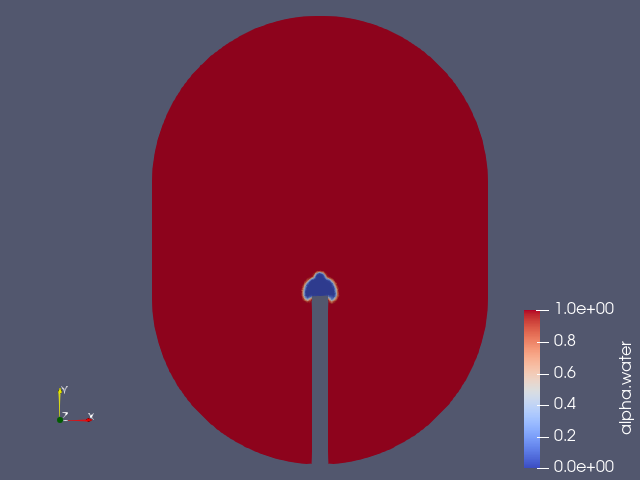
\includegraphics[width=\textwidth]{images/alphawater_28.png}
        \caption{\centering }
    \end{subfigure}
    \hspace{1cm}
    \begin{subfigure}{.45\textwidth}
        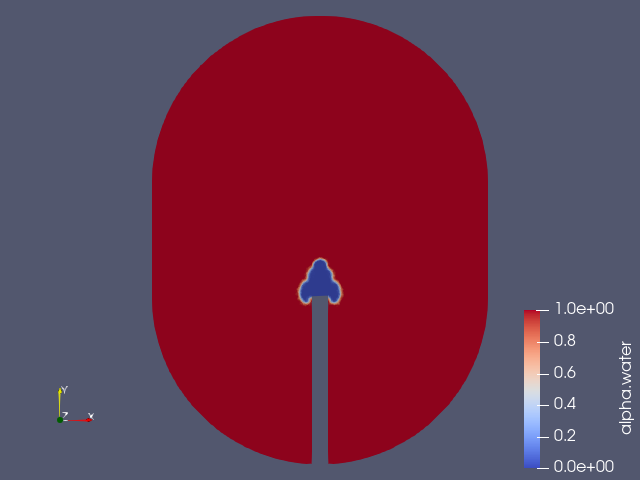
\includegraphics[width=\textwidth]{images/alphawater_88.png}
        \caption{\centering }
    \end{subfigure}
    
    % Second row
    \vspace{1em} % Space between rows
    \begin{subfigure}{.45\textwidth}
        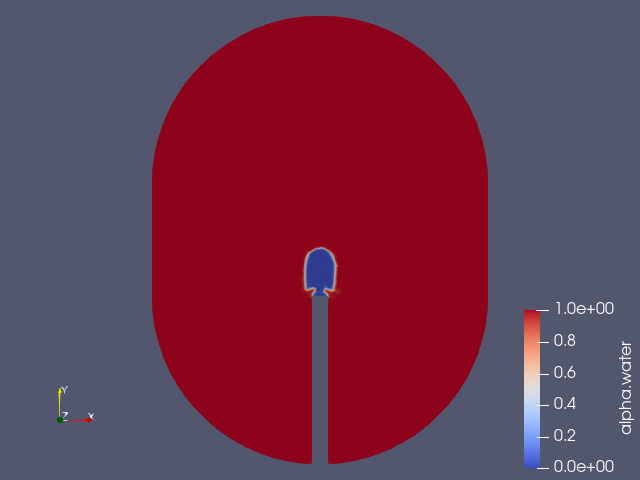
\includegraphics[width=\textwidth]{images/alphawater_175.png}
        \caption{\centering }
    \end{subfigure}
    \hspace{1cm}
    \begin{subfigure}{.45\textwidth}
        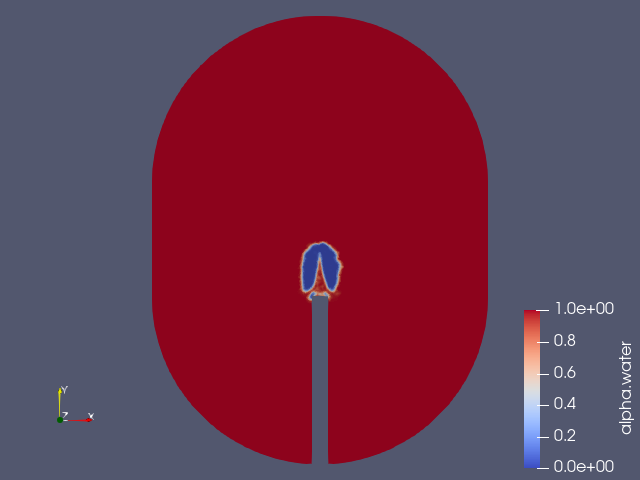
\includegraphics[width=\textwidth]{images/alphawater_198.png}
        \caption{\centering }
    \end{subfigure}

    % Third row
    \vspace{1em} % Space between rows
    \begin{subfigure}{.45\textwidth}
        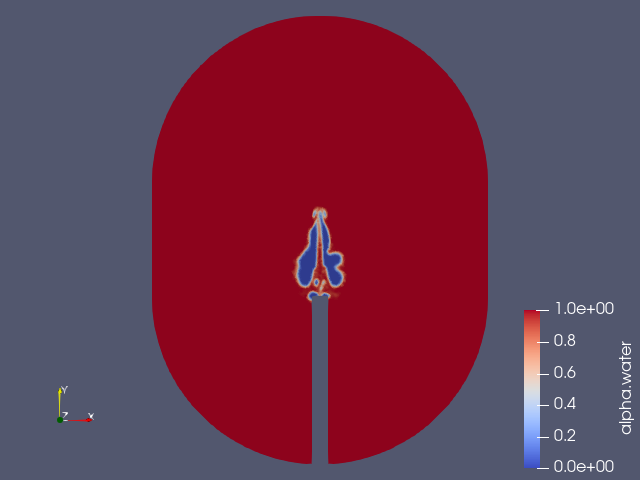
\includegraphics[width=\textwidth]{images/alphawater_254.png}
        \caption{\centering }
    \end{subfigure}
    \hspace{1cm}
    \begin{subfigure}{.45\textwidth}
        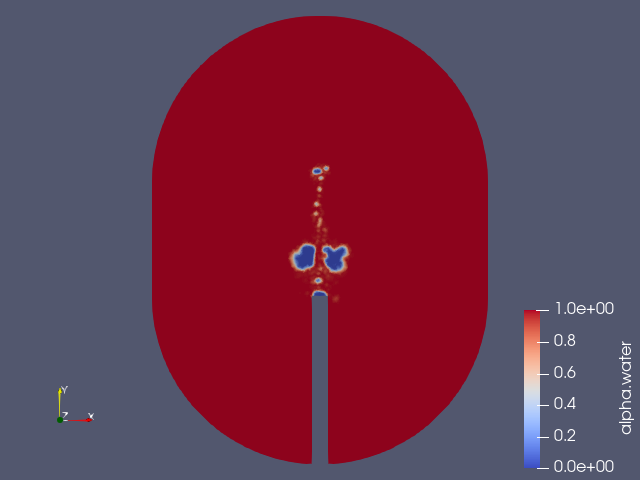
\includegraphics[width=\textwidth]{images/alphawater_365.png}
        \caption{\centering }
    \end{subfigure}

    \hspace{5pt}
    \caption{\centering Распределение фаз (синий цвет -- пар, красный -- вода) в процессе роста каскадного кавитационного пузыря, вызванного тройным лазерным импульсом, в различные моменты времени $t$}
    \label{fig:triple_impulse_alphawater}
\end{figure}

При использовании тройного лазерного импульса динамика пузыря оказалась более сложной. 
На рисунках~\ref{fig:triple_impulse_alphawater}, ~\ref{fig:triple_impulse_pressure}, ~\ref{fig:triple_impulse_velocity} представлены распределения фаз, давления и модуля скорости в моделировании при $p_1 = 1.8 \cdot 10^6$ Па, $p_2 = 2p_1$, $p_3 = 4p_1$.
Первый импульс инициировал формирование пузыря, в то время как последующие взаимодействовали с уже растущим пузырем. 
Это приводило к появлению интересных эффектов, таких как удлинение пузыря или его асимметричный коллапс, зависящих от времени и энергии следующих импульсов. 
Подобные результаты особенно важны для применения в задачах, где используются несколько импульсов, например, в высокоточных лазерных хирургических процедурах или промышленных процессах очистки.

\begin{figure}[h!]
    \centering
    % First row
    \begin{subfigure}{.45\textwidth}
        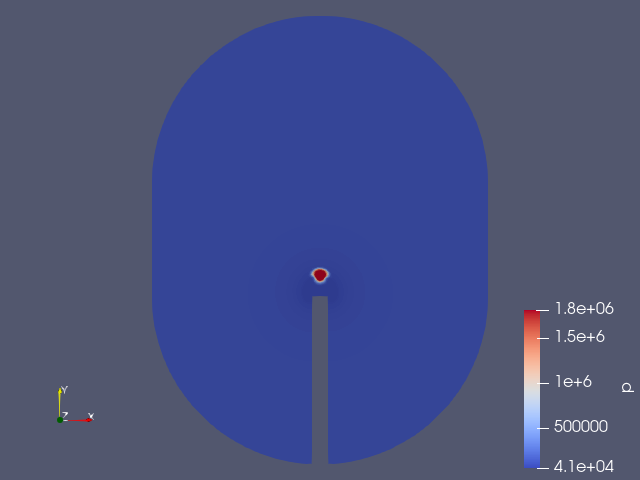
\includegraphics[width=\textwidth]{images/pressure_10.png}
        \caption{\centering }
    \end{subfigure}
    \hspace{1cm}
    \begin{subfigure}{.45\textwidth}
        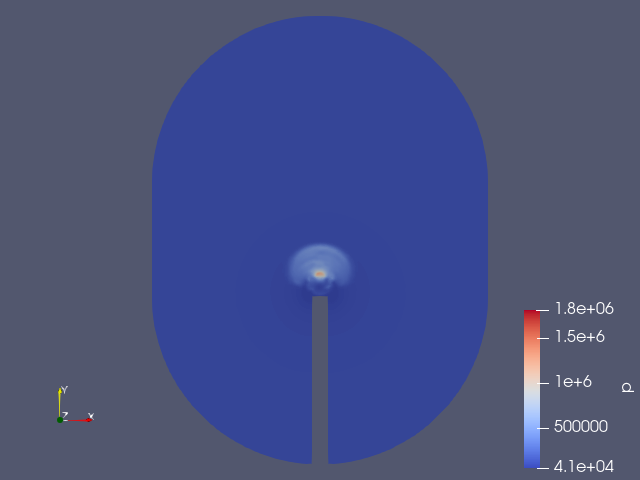
\includegraphics[width=\textwidth]{images/pressure_15.png}
        \caption{\centering }
    \end{subfigure}
    
    % Second row
    \vspace{1em} % Space between rows
    \begin{subfigure}{.45\textwidth}
        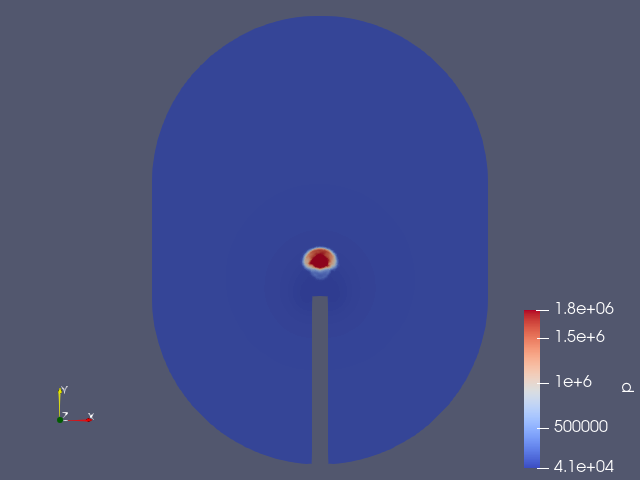
\includegraphics[width=\textwidth]{images/pressure_61.png}
        \caption{\centering }
    \end{subfigure}
    \hspace{1cm}
    \begin{subfigure}{.45\textwidth}
        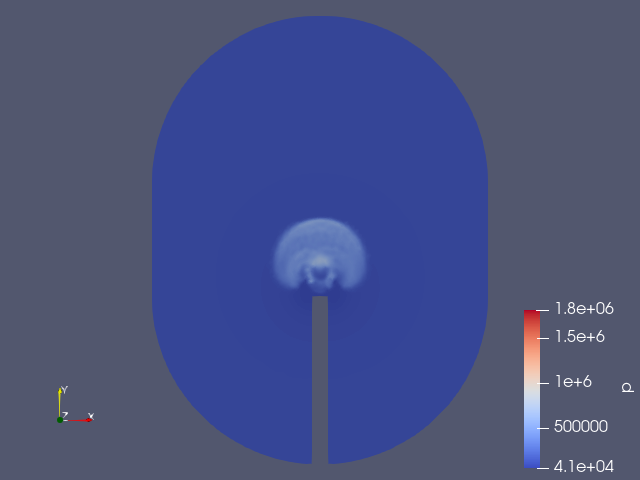
\includegraphics[width=\textwidth]{images/pressure_68.png}
        \caption{\centering }
    \end{subfigure}

    \hspace{5pt}
    \caption{\centering Распределение давления в процессе роста каскадного кавитационного пузыря, вызванного тройным лазерным импульсом, в различные моменты времени $t$}
    \label{fig:triple_impulse_pressure}
\end{figure}


\begin{figure}[h!]
    \centering
    % First row
    \begin{subfigure}{.45\textwidth}
        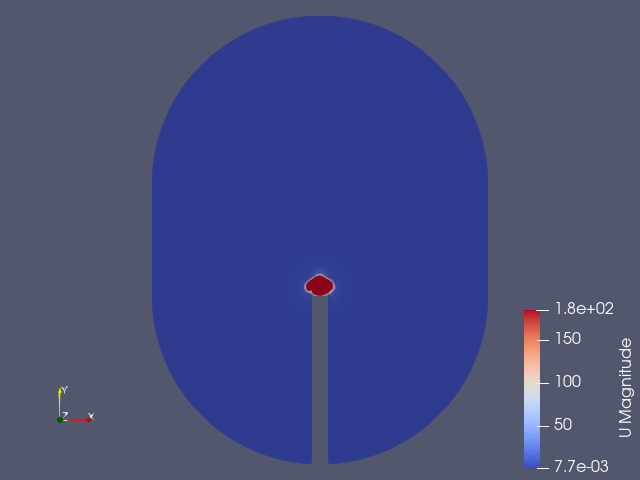
\includegraphics[width=\textwidth]{images/velocity_15.png}
        \caption{\centering }
    \end{subfigure}
    \hspace{1cm}
    \begin{subfigure}{.45\textwidth}
        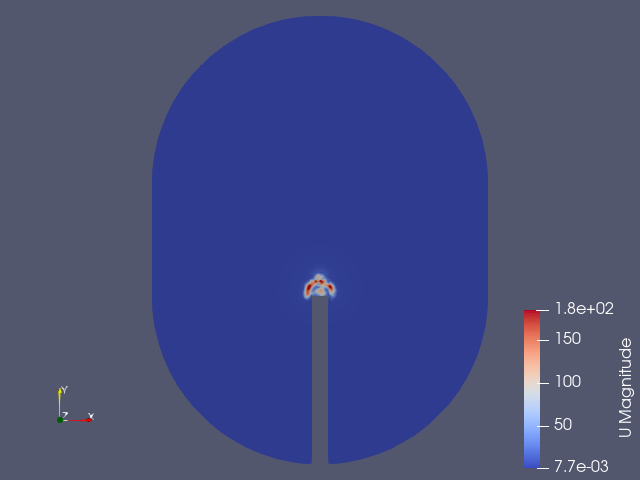
\includegraphics[width=\textwidth]{images/velocity_32.png}
        \caption{\centering }
    \end{subfigure}
    
    % Second row
    \vspace{1em} % Space between rows
    \begin{subfigure}{.45\textwidth}
        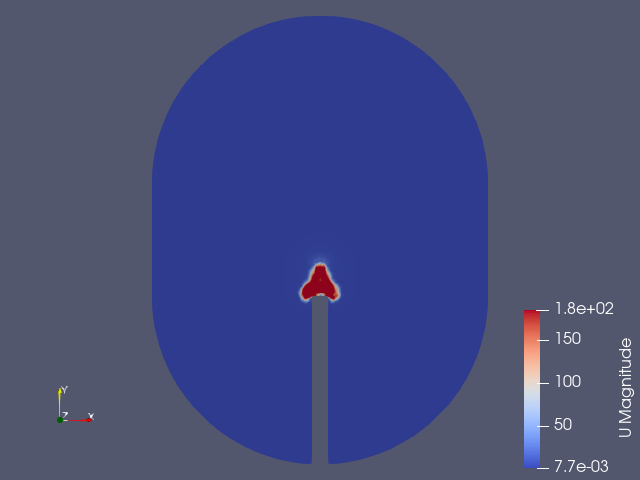
\includegraphics[width=\textwidth]{images/velocity_78.png}
        \caption{\centering }
    \end{subfigure}
    \hspace{1cm}
    \begin{subfigure}{.45\textwidth}
        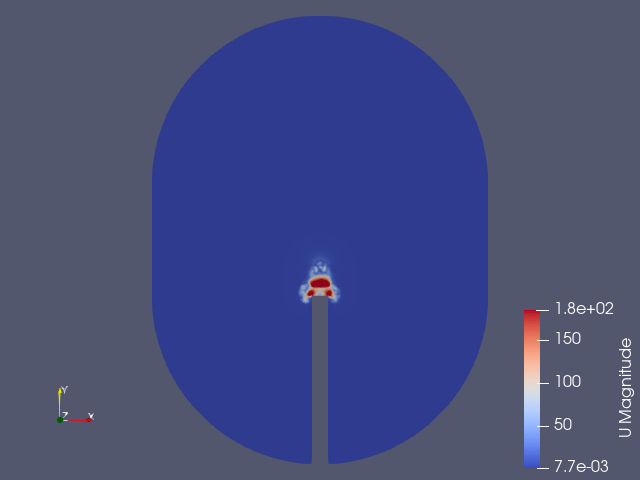
\includegraphics[width=\textwidth]{images/velocity_85.png}
        \caption{\centering }
    \end{subfigure}

    \hspace{5pt}
    \caption{\centering Распределение модуля скорости в процессе роста каскадного кавитационного пузыря, вызванного тройным лазерным импульсом, в различные моменты времени $t$}
    \label{fig:triple_impulse_velocity}
\end{figure}

Распредение давления и скорости при росте каскадного кавитационного пузыря дает более детальное представление о протекании процесса.
На рисунках~\ref{fig:triple_impulse_pressure} и~\ref{fig:triple_impulse_velocity} видно, что в момент воздействия инициирующего импульса в зоне кавитации наблюдается резкий градиент давлений, достигающий $\triangle p \sim 10^2 \text{ Па}$, и значительные локальные скорости течения порядка $10^2 \text{ м/с}$, что на несколько порядков превышает параметры невозмущенной жидкости.
Последующая стадия релаксации системы сопровождается сложным взаимодействием между вновь образованной кавитационной полостью с ранее существовавшими пузырями и окружающей жидкой средой.
В результате указанных взаимодействий, а также диссипации энергии и массообмена происходит постепенная стабилизация системы.
В ходе этого процесса наблюдаются: нелинейная динамика межфазных границ, генерация ударных волн при коллапсе вторичных пузырей (рисунок~\ref{fig:triple_impulse_pressure} б, г), турбулентное перемешивание в пограничных слоях. 
По окончании релаксации все параметры имеют равномерное распределение.

Для сравнения динамик кавитационного пузыря в эксперименте и в моделировании был проведен расчет нормированных площадей газовой фазы от времени в эксперименте и в моделировании (рисунки~\ref{fig:sim_gas}, ~\ref{fig:exp_sim}).

\begin{figure}[h!]
    \centering
    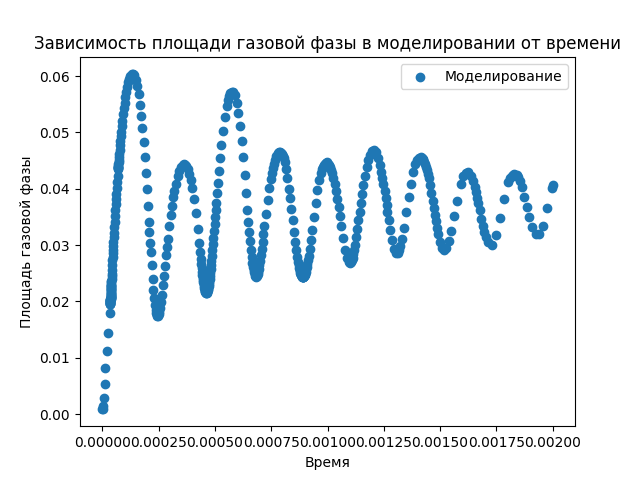
\includegraphics[width=0.7\linewidth]{images/sim_gas.png}
    \caption{\centering Зависимость площади газовой фазы от времени в моделировании}
    \label{fig:sim_gas}
\end{figure}

\begin{figure}[h!]
    \centering
    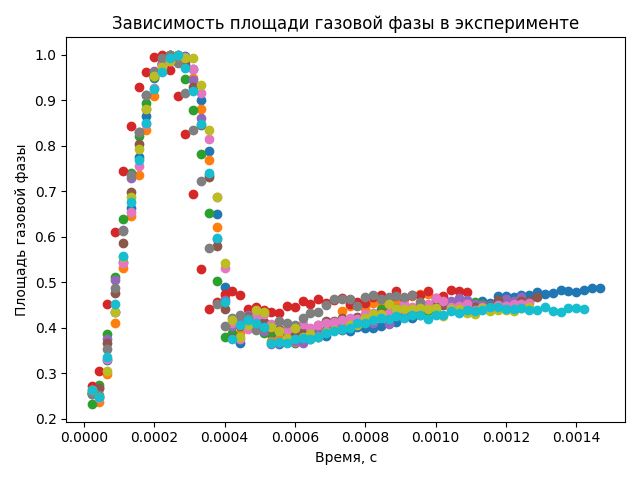
\includegraphics[width=0.7\linewidth]{images/exp_all.png}
    \caption{\centering Зависимость площади газовой фазы от времени в эксперименте}
    \label{fig:exp_sim}
\end{figure}

На рисунке~\ref{fig:sim_gas} отчетливо видно, что при моделировании кавитационный процесс имеет явный осциллирующий характер, даже после прекращения лазерного воздействия.
При этом, из рисунка~\ref{fig:exp_sim} следует, что при экспериментальном изучении кавитации наблюдается единственный пик на графике площади газовой фазы, после чего зависимость выходит на постоянное значение, что может быть обусловлено недостаточным временем наблюдения эксперимента для полной релаксации системы и растворении кавитационного пузыря.